\documentclass[12pt,a4paper]{article}

% === ENCODAGE ET LANGUE ===
\usepackage[utf8]{inputenc}
\usepackage[T1]{fontenc}
\usepackage[french]{babel}

% === MISE EN PAGE ===
\usepackage{geometry}
\geometry{margin=2.5cm}
\usepackage{setspace}
\onehalfspacing

% === POLICES ET TYPOGRAPHIE ===
\usepackage{lmodern}
\usepackage{microtype}

% === GRAPHIQUES ET FIGURES ===
\usepackage{graphicx}
\graphicspath{{results/}}
\usepackage{tikz}
\usetikzlibrary{arrows.meta, shapes.geometric, positioning, calc, fit, backgrounds}
\usepackage{pgfplots}
\pgfplotsset{compat=1.18}
\usepackage{float}

% === TABLEAUX ===
\usepackage{booktabs}
\usepackage{multirow}
\usepackage{tabularx}
\usepackage{array}
\usepackage{colortbl}

% === COULEURS ===
\usepackage[table]{xcolor}
\definecolor{upsred}{RGB}{180, 30, 40}
\definecolor{criticalred}{RGB}{220, 53, 69}
\definecolor{importantyellow}{RGB}{255, 193, 7}
\definecolor{moderategray}{RGB}{108, 117, 125}
\definecolor{lightgray}{RGB}{245, 245, 245}
\definecolor{codebg}{RGB}{248, 249, 250}

% === MATHS ===
\usepackage{amsmath}
\usepackage{amssymb}

% === LISTINGS (CODE) ===
\usepackage{listings}
\lstset{
  basicstyle=\ttfamily\small,
  backgroundcolor=\color{codebg},
  frame=single,
  rulecolor=\color{gray!30},
  breaklines=true,
  columns=fullflexible,
  literate={é}{{\'e}}1 {è}{{\`e}}1 {ê}{{\^e}}1 {à}{{\`a}}1 {ù}{{\`u}}1 {û}{{\^u}}1 {ç}{{\c{c}}}1 {ô}{{\^o}}1 {î}{{\^i}}1
}

% === LIENS ===
\usepackage{hyperref}
\hypersetup{
  colorlinks=true,
  linkcolor=upsred,
  citecolor=upsred,
  urlcolor=blue!70!black,
  pdfauthor={Mohamed DIALLO et al.},
  pdftitle={GeoR2LLMs -- Rapport de travail Phase 1},
  pdfsubject={Système Question-Réponse Géographique avec RAG}
}

% === BIBLIOGRAPHIE ===
\usepackage{cite}

% === EN-TÊTES ET PIEDS DE PAGE ===
\usepackage{fancyhdr}
\pagestyle{fancy}
\fancyhf{}
\fancyhead[L]{\small\textit{GeoR2LLMs -- Rapport de travail Phase 1}}
\fancyhead[R]{\small\textit{M2 IA -- UPS}}
\fancyfoot[C]{\thepage}
\renewcommand{\headrulewidth}{0.4pt}
\renewcommand{\footrulewidth}{0.4pt}

\fancypagestyle{plain}{
  \fancyhf{}
  \fancyfoot[C]{\thepage}
  \renewcommand{\headrulewidth}{0pt}
  \renewcommand{\footrulewidth}{0pt}
}

% === TITRES ===
\usepackage{titlesec}
\titleformat{\section}{\Large\bfseries\color{upsred}}{\thesection}{1em}{}
\titleformat{\subsection}{\large\bfseries}{\thesubsection}{1em}{}
\titleformat{\subsubsection}{\normalsize\bfseries\itshape}{\thesubsubsection}{1em}{}

% === ENUMÉRATION ===
\usepackage{enumitem}

% === CAPTION ===
\usepackage{caption}
\captionsetup{font=small, labelfont=bf, format=hang}

% ====================================================================
\begin{document}

% ====================================================================
% PAGE DE GARDE
% ====================================================================
\begin{titlepage}
  \centering
  \vspace*{1cm}

  {\Large\textsc{Université Toulouse III -- Paul Sabatier}}\\[0.3cm]
  {\large\textsc{Master 2 Intelligence Artificielle}}\\[0.2cm]
  {\normalsize IRIT -- Institut de Recherche en Informatique de Toulouse}\\[2cm]

  \rule{\textwidth}{1.5pt}\\[0.6cm]
  {\huge\bfseries Système Question-Réponse\\[0.3cm] en Géographie avec RAG}\\[0.4cm]
  {\Large\textit{Rapport de travail -- Phase 1 : Plateforme de base}}\\[0.3cm]
  {\large Projet GeoR2LLMs}\\[0.4cm]
  \rule{\textwidth}{1.5pt}\\[2cm]

  \begin{minipage}{0.45\textwidth}
    \begin{flushleft}
      \textbf{Réalisé par :}\\[0.3cm]
      Mohamed DIALLO\\
      Hiba L'MOUDDEN\\
      Feras MAKHLOUF\\
      Osama BAAZZI\\
      Ousama BOUTEZROUT
    \end{flushleft}
  \end{minipage}
  \hfill
  \begin{minipage}{0.45\textwidth}
    \begin{flushright}
      \textbf{Sous la direction de :}\\[0.3cm]
      Madame Lynda TAMINE-LECHANI\\
      Professeure -- IRIT\\[0.5cm]
      \textbf{UE :} Chef d'\oe uvre\\
      \textbf{Année :} 2025--2026
    \end{flushright}
  \end{minipage}

  \vfill

  {\large Février 2026}
\end{titlepage}

% ====================================================================
% TABLE DES MATIÈRES
% ====================================================================
\newpage
\tableofcontents
\newpage

% ====================================================================
% 1. INTRODUCTION
% ====================================================================
\section{Introduction}
\label{sec:introduction}

Le projet GeoR2LLMs (\textit{Geographic Retrieval-augmented generation with Large Language Models}) s'inscrit dans le cadre du chef-d'\oe uvre du Master 2 Intelligence Artificielle de l'Université Toulouse III -- Paul Sabatier, sous la direction de Madame Lynda Tamine-Lechani à l'IRIT. Ce rapport de travail documente l'implémentation et les résultats de la Phase 1 du projet.

\subsection{Contexte et motivations}

Le Question-Réponse géographique (GeoQA) constitue un défi particulier pour les systèmes de traitement automatique des langues. Mai et al.~\cite{mai_geographic_2021} identifient les questions géographiques comme nécessitant un raisonnement spatial, la compréhension de relations topologiques et l'intégration de connaissances spécifiques au domaine. Cohn et Blackwell~\cite{cohn_evaluating_2024} montrent qu'aucun LLM actuel ne parvient à raisonner de manière fiable sur les directions cardinales, même avec une température de zéro.

L'architecture RAG (\textit{Retrieval-Augmented Generation}), introduite par Lewis et al.~\cite{lewis2020retrieval} dans le cadre de NeurIPS 2020, propose d'augmenter les LLMs avec des connaissances externes récupérées dynamiquement depuis un corpus. Gao et al.~\cite{gao2023ragsurvey} proposent une taxonomie des systèmes RAG distinguant le RAG na\"if (retrieve-then-read) du RAG avancé (avec réécriture de requêtes ou re-ranking). Notre implémentation suit l'approche na\"ive.

\subsection{Objectif de la Phase 1}

La Phase 1 du projet vise à mettre en place une \textbf{plateforme de base} pour le système GeoQA-RAG, conformément au cahier des charges. Les objectifs sont :
\begin{enumerate}[leftmargin=*]
  \item Implémenter un pipeline RAG complet avec les composants spécifiés (Qwen3-0.6B, BGE-m3, FAISS)
  \item Établir une baseline (LLM seul, sans RAG) comme point de comparaison
  \item Évaluer l'apport du RAG sur le dataset GeoSQA~\cite{huang_geosqa_2019}
  \item Mesurer la qualité du retrieval indépendamment de la génération
\end{enumerate}

\subsection{Organisation du rapport}

La section~\ref{sec:architecture} présente l'architecture du système. La section~\ref{sec:methodologie} détaille les choix méthodologiques. Les résultats expérimentaux sont rapportés en section~\ref{sec:resultats} et analysés en section~\ref{sec:analyse}. La section~\ref{sec:conclusion} conclut et ouvre sur la Phase 2.

% ====================================================================
% 2. ARCHITECTURE DU SYSTÈME
% ====================================================================
\section{Architecture du système}
\label{sec:architecture}

Le système repose sur une architecture RAG composée de trois modules : un \textbf{Retriever}, un \textbf{Generator} et un \textbf{Evaluator}. La figure~\ref{fig:architecture} illustre le pipeline.

\begin{figure}[H]
\centering
\resizebox{\textwidth}{!}{%
\begin{tikzpicture}[
  node distance=1.2cm and 2cm,
  box/.style={rectangle, draw, rounded corners=4pt, minimum height=1.2cm, minimum width=3cm, align=center, font=\small},
  data/.style={box, fill=blue!8, draw=blue!40},
  process/.style={box, fill=green!8, draw=green!40},
  model/.style={box, fill=orange!10, draw=orange!40},
  result/.style={box, fill=red!8, draw=red!40},
  arrow/.style={-{Stealth[length=3mm]}, thick, draw=gray!70},
  lbl/.style={font=\scriptsize\itshape, text=gray}
]

% Données d'entrée
\node[data] (wiki) {Wikipedia FR\\{\scriptsize 300 articles}};
\node[data, below=0.8cm of wiki] (question) {Question\\{\scriptsize GeoSQA}};

% Retriever
\node[process, right=2cm of wiki] (chunking) {Chunking\\{\scriptsize 512 car., overlap 50}};
\node[model, right=1.5cm of chunking] (bge) {BGE-m3\\{\scriptsize 1024 dim.}};
\node[process, right=1.5cm of bge] (faiss) {FAISS\\{\scriptsize IndexFlatIP}};

% Generator
\node[model, right=2cm of question] (embed_q) {Encodage\\{\scriptsize question}};
\node[process, right=3.7cm of embed_q] (topk) {Top-K\\{\scriptsize K=5}};
\node[model, below=2cm of faiss] (qwen) {Qwen3-0.6B\\{\scriptsize Generator}};
\node[result, right=1.5cm of qwen] (reponse) {Réponse\\{\scriptsize générée}};

% Flèches corpus
\draw[arrow] (wiki) -- (chunking);
\draw[arrow] (chunking) -- (bge);
\draw[arrow] (bge) -- node[above, lbl] {embeddings} (faiss);

% Flèches question
\draw[arrow] (question) -- (embed_q);
\draw[arrow] (embed_q) -- node[above, lbl] {vecteur requête} (topk);
\draw[arrow] (faiss) -- node[right, lbl] {index} (topk);

% Flèches génération
\draw[arrow] (topk) -- node[right, lbl] {contexte} (qwen);
\draw[arrow] (question.south) |- (qwen.west);
\draw[arrow] (qwen) -- (reponse);

% Cadres
\begin{scope}[on background layer]
  \node[fit=(chunking)(bge)(faiss), draw=green!60, dashed, rounded corners=8pt, inner sep=10pt, label={[font=\small\bfseries, text=green!60!black]above:Module Retriever}] {};
  \node[fit=(qwen)(reponse), draw=orange!60, dashed, rounded corners=8pt, inner sep=10pt, label={[font=\small\bfseries, text=orange!60!black]below:Module Generator}] {};
\end{scope}

\end{tikzpicture}
}
\caption{Architecture du pipeline RAG. Le corpus Wikipedia est découpé en chunks, encodé par BGE-m3 et indexé dans FAISS. Les questions sont encodées puis les top-K passages récupérés sont fournis comme contexte au générateur Qwen3-0.6B.}
\label{fig:architecture}
\end{figure}

\subsection{Module Retriever}

Le retriever utilise le modèle d'embeddings multilingue \textbf{BGE-m3} (BAAI), présenté par Chen et al.~\cite{chen2024bgem3} à ACL 2024 Findings. BGE-m3 produit des vecteurs denses de 1024 dimensions et supporte plus de 100 langues. Les documents sont encodés et stockés dans un index \textbf{FAISS}~\cite{johnson2019faiss} (\texttt{IndexFlatIP}) utilisant le produit scalaire après normalisation L2, équivalent à la similarité cosinus. Pour une requête $q$, le retriever retourne les $K$ passages les plus similaires :
\begin{equation}
  \text{Top-K}(q) = \underset{d_i \in \mathcal{C}}{\text{argmax-K}} \; \cos(\mathbf{e}_q, \mathbf{e}_{d_i})
\end{equation}
où $\mathbf{e}_q$ et $\mathbf{e}_{d_i}$ sont les embeddings de la requête et du document, et $\mathcal{C}$ est le corpus de chunks.

\subsection{Module Generator}

Le générateur est basé sur \textbf{Qwen3-0.6B}~\cite{yang2025qwen3}, un modèle de langage de 0.6 milliard de paramètres de la famille Qwen3 (Alibaba). Selon le rapport technique Qwen3, ce modèle supporte un mode \textit{thinking} activable. Nous l'utilisons avec \texttt{enable\_thinking=False} pour obtenir des réponses directes. Le prompt est structuré via le template de chat Qwen3 :

\begin{lstlisting}[language=Python, caption={Prompt template pour le mode RAG}]
system: "Tu es un expert en geographie. Reponds
         uniquement avec la lettre correcte."
user:   "Contexte: {documents recuperes}
         Question: {question}
         Options: A) ... B) ... C) ... D) ..."
\end{lstlisting}

En mode \textbf{baseline}, aucun contexte n'est fourni : le modèle répond uniquement à partir de ses connaissances internes.

\subsection{Module Evaluator}

L'évaluateur mesure la performance selon deux axes, conformément aux métriques standard du QA~\cite{rajpurkar2016squademnlp} :
\begin{itemize}[leftmargin=*]
  \item \textbf{Qualité de génération} : Accuracy MCQ, Exact Match, F1 token-level, Contains
  \item \textbf{Qualité de retrieval} : Hit Rate@K, MRR@K (métriques classiques en recherche d'information~\cite{karpukhin2020dense})
\end{itemize}

% ====================================================================
% 3. MÉTHODOLOGIE
% ====================================================================
\section{Méthodologie}
\label{sec:methodologie}

\subsection{Configuration expérimentale}

Le tableau~\ref{tab:config} résume l'ensemble des hyperparamètres et composants du système, tels qu'enregistrés dans le fichier \texttt{phase1\_metrics.json} produit par le notebook.

\begin{table}[H]
\centering
\caption{Configuration du système GeoR2LLMs -- Phase 1}
\label{tab:config}
\begin{tabular}{@{} l l l @{}}
\toprule
\textbf{Catégorie} & \textbf{Paramètre} & \textbf{Valeur} \\
\midrule
\multirow{5}{*}{\textbf{Génération}}
  & Modèle LLM & Qwen/Qwen3-0.6B \\
  & Temperature & 0.7 \\
  & Top-p (nucleus) & 0.8 \\
  & Top-k (sampling) & 20 \\
  & Max tokens générés & 100 \\
\midrule
\multirow{4}{*}{\textbf{Retrieval}}
  & Modèle embeddings & BAAI/bge-m3 (1024 dim.) \\
  & Index vectoriel & FAISS IndexFlatIP \\
  & Taille des chunks & 512 caractères \\
  & Chevauchement (overlap) & 50 caractères \\
\midrule
\multirow{2}{*}{\textbf{Dataset}}
  & Benchmark & rfr2003/Geo\_Benchmark \\
  & Configuration & GeoSQA (test split) \\
\midrule
\multirow{3}{*}{\textbf{Corpus}}
  & Source & wikimedia/wikipedia \\
  & Version & 20231101.fr \\
  & Nombre d'articles & 300 \\
\midrule
\textbf{Environnement} & GPU & Google Colab -- NVIDIA T4 (16 Go) \\
\bottomrule
\end{tabular}
\end{table}

\subsection{Dataset : GeoSQA}

GeoSQA~\cite{huang_geosqa_2019} est un benchmark de question-réponse scénarisé en géographie, développé par Huang et al. à l'Université de Nanjing et présenté à EMNLP-IJCNLP 2019. Le dataset contient \textbf{1\,981 scénarios} et \textbf{4\,110 questions à choix multiples} au niveau lycée chinois, où les diagrammes ont été annotés en descriptions textuelles. Chaque question comprend :
\begin{itemize}[leftmargin=*]
  \item Un \textbf{scénario} contextuel (description de situation géographique)
  \item La \textbf{question} associée
  \item \textbf{4 options} (A, B, C, D)
  \item La \textbf{réponse correcte} (une lettre)
\end{itemize}

Le split de test contient \textbf{838 questions}. L'évaluation porte sur un sous-ensemble de \textbf{200 questions} échantillonnées aléatoirement, pour des raisons de temps d'exécution sur Google Colab.

\paragraph{Langue des questions.} Les questions GeoSQA sont originellement en chinois et ont été traduites en anglais dans la version HuggingFace (\texttt{rfr2003/Geo\_Benchmark}). Notre corpus est constitué d'articles Wikipédia en français, créant un décalage linguistique entre les questions et le corpus.

\subsection{Corpus : Wikipedia français}

Le corpus est constitué de \textbf{300 articles} chargés en streaming depuis le dump Wikipedia français (\texttt{wikimedia/wikipedia}, configuration \texttt{20231101.fr}). Chaque article est découpé en chunks de 512 caractères avec un chevauchement de 50 caractères, produisant un total de \textbf{2\,527 chunks} (valeur mesurée lors de l'exécution).

\subsection{Protocole d'évaluation}

\subsubsection{Métriques de génération}

Les métriques de génération suivent les conventions établies par Rajpurkar et al.~\cite{rajpurkar2016squademnlp} pour le benchmark SQuAD :

\begin{itemize}[leftmargin=*]
  \item \textbf{Accuracy (MCQ)} : Proportion de questions où la lettre prédite correspond à la lettre correcte.
  \begin{equation}
    \text{Accuracy} = \frac{1}{N} \sum_{i=1}^{N} \mathbb{1}[\hat{y}_i = y_i]
  \end{equation}

  \item \textbf{Exact Match (EM)} : Correspondance exacte entre le texte prédit (normalisé) et le texte de la réponse correcte.

  \item \textbf{F1 Score} : F1 au niveau des tokens entre la prédiction et la référence, après tokenisation et normalisation.
  \begin{equation}
    F_1 = \frac{2 \cdot P \cdot R}{P + R}, \quad P = \frac{|\hat{T} \cap T|}{|\hat{T}|}, \quad R = \frac{|\hat{T} \cap T|}{|T|}
  \end{equation}
  où $\hat{T}$ et $T$ sont les ensembles de tokens de la prédiction et de la référence.

  \item \textbf{Contains} : Proportion de cas où les mots-clés de la réponse correcte apparaissent dans la prédiction.
\end{itemize}

\subsubsection{Métriques de retrieval}

Les métriques de retrieval suivent les conventions du \textit{Dense Passage Retrieval} (DPR) de Karpukhin et al.~\cite{karpukhin2020dense} :

\begin{itemize}[leftmargin=*]
  \item \textbf{Hit Rate@K} : Proportion de questions pour lesquelles au moins un des $K$ documents récupérés contient le texte de la réponse correcte.
  \begin{equation}
    \text{HR@K} = \frac{1}{N} \sum_{i=1}^{N} \mathbb{1}\left[\exists j \leq K : y_i \in d_j^{(i)}\right]
  \end{equation}

  \item \textbf{MRR@K} (\textit{Mean Reciprocal Rank}) : Moyenne du rang réciproque du premier document pertinent parmi les top-K.
  \begin{equation}
    \text{MRR@K} = \frac{1}{N} \sum_{i=1}^{N} \frac{1}{\text{rank}_i}
  \end{equation}
\end{itemize}

% ====================================================================
% 4. RÉSULTATS EXPÉRIMENTAUX
% ====================================================================
\section{Résultats expérimentaux}
\label{sec:resultats}

Tous les résultats présentés dans cette section sont issus de l'exécution du notebook \texttt{Phase1\_GeoR2LLMs.ipynb} sur Google Colab (GPU T4). Les valeurs numériques sont extraites du fichier \texttt{phase1\_metrics.json} et les prédictions détaillées du fichier \texttt{phase1\_predictions.csv}, tous deux générés automatiquement par le notebook.

\subsection{Comparaison Baseline vs RAG}

Le tableau~\ref{tab:results_main} présente les résultats de l'évaluation sur 200 questions GeoSQA.

\begin{table}[H]
\centering
\caption{Résultats Baseline vs RAG sur GeoSQA (200 questions). Valeurs issues de \texttt{phase1\_metrics.json}.}
\label{tab:results_main}
\begin{tabular}{@{} l c c c @{}}
\toprule
\textbf{Métrique} & \textbf{Baseline} & \textbf{RAG} & \textbf{Delta} \\
\midrule
Accuracy (MCQ) & 0.270 & 0.290 & \textcolor{green!60!black}{+0.020} \\
Exact Match & 0.000 & 0.000 & 0.000 \\
F1 Score & 0.028 & 0.016 & \textcolor{red}{--0.013} \\
Contains & 0.025 & 0.035 & \textcolor{green!60!black}{+0.010} \\
\midrule
Temps (secondes) & 341 & 473 & +132 \\
\bottomrule
\end{tabular}
\end{table}

La figure~\ref{fig:baseline_vs_rag} illustre cette comparaison. Ce graphique est produit directement par le notebook lors de l'exécution.

\begin{figure}[H]
\centering

\includegraphics[width=0.9\textwidth]{fig1_baseline_vs_rag.png}
\caption{Comparaison des métriques de génération entre le mode Baseline (LLM seul) et le mode RAG (LLM + Wikipedia). Graphique généré par le notebook \texttt{Phase1\_GeoR2LLMs.ipynb}.}
\label{fig:baseline_vs_rag}
\end{figure}

\subsection{Métriques de retrieval}

Le tableau~\ref{tab:retrieval} et la figure~\ref{fig:retrieval} présentent les performances du module de retrieval.

\begin{table}[H]
\centering
\caption{Métriques de retrieval (BGE-m3 + FAISS). Valeurs issues de \texttt{phase1\_metrics.json}.}
\label{tab:retrieval}
\begin{tabular}{@{} l c @{}}
\toprule
\textbf{Métrique} & \textbf{Score} \\
\midrule
Hit Rate@1 & 0.040 \\
Hit Rate@3 & 0.060 \\
Hit Rate@5 & 0.080 \\
MRR@5 & 0.053 \\
\bottomrule
\end{tabular}
\end{table}

\begin{figure}[H]
\centering
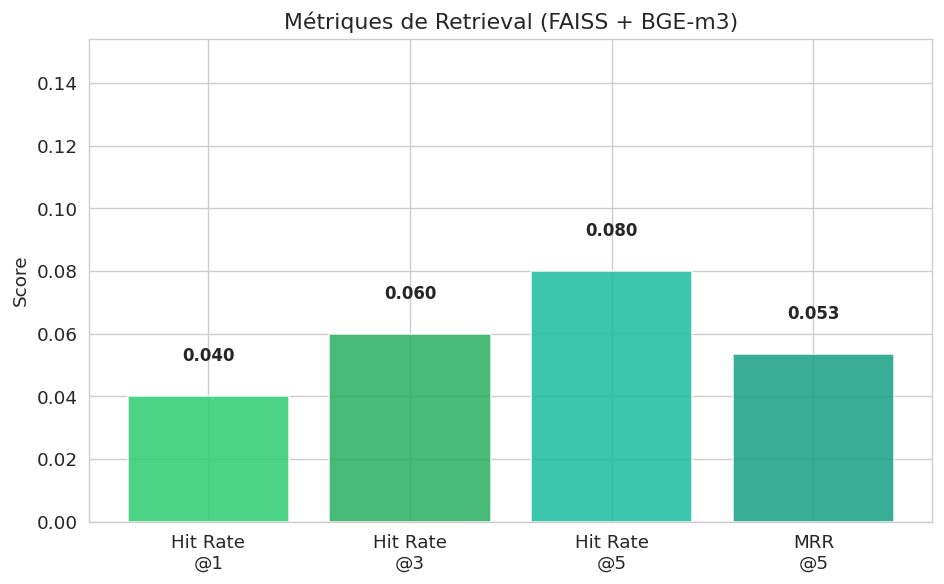
\includegraphics[width=0.75\textwidth]{fig2_retrieval_metrics.png}
\caption{Métriques de retrieval (Hit Rate@K et MRR@5). Graphique généré par le notebook.}
\label{fig:retrieval}
\end{figure}

\subsection{Distribution des scores F1}

La figure~\ref{fig:f1_distribution} montre la distribution des scores F1 par question, en mode Baseline et en mode RAG. La grande majorité des scores F1 sont concentrés à 0.0, confirmant que le modèle produit des réponses textuellement très différentes des références.

\begin{figure}[H]
\centering

\includegraphics[width=\textwidth]{fig3_f1_distribution.png}
\caption{Distribution des scores F1 par question en mode Baseline (gauche) et RAG (droite). La ligne rouge indique la moyenne. Graphique généré par le notebook.}
\label{fig:f1_distribution}
\end{figure}

\subsection{Analyse qualitative des prédictions}

Le tableau~\ref{tab:examples} présente des exemples de prédictions extraits du fichier \texttt{phase1\_predictions.csv}.

\begin{table}[H]
\centering
\caption{Exemples de prédictions extraits de \texttt{phase1\_predictions.csv}}
\label{tab:examples}
\small
\begin{tabularx}{\textwidth}{@{} p{0.6cm} X c c c @{}}
\toprule
\textbf{\#} & \textbf{Question (résumée)} & \textbf{Vérité} & \textbf{Base.} & \textbf{RAG} \\
\midrule
0 & \textit{``While Tiangong-1 and Shenzhou-9 [\ldots] same level as?''} & D & D & D \\
\rowcolor{lightgray}
1 & \textit{``When Tiangong-1 and Shenzhou-9 docked, which city had longest daylight?''} & A & A & A \\
2 & \textit{``Statement about Tiangong-1 [\ldots] during orbit is incorrect?''} & B & A & A \\
\rowcolor{lightgray}
7 & \textit{``Shouguang's vegetable production [\ldots] upstream enterprises?''} & B & A & A \\
24 & \textit{``Trends in Shandong Province's socioeconomic development?''} & B & B & B \\
\bottomrule
\end{tabularx}
\end{table}

\paragraph{Observations qualitatives issues des prédictions.} L'examen du fichier \texttt{phase1\_predictions.csv} (200 lignes) révèle :

\begin{enumerate}[leftmargin=*]
  \item \textbf{Mélange linguistique} : Le modèle produit des réponses en français alors que les questions sont en anglais. Par exemple, pour la question \#0 en anglais sur Tiangong-1, la réponse RAG est : \textit{``La réponse est : le système céleste avec laquelle Tiangong-1 et Shenzhou-9 forment.''}.

  \item \textbf{Verbosité} : Au lieu de répondre par la lettre seule, le modèle génère des phrases complètes (ex. question \#7 : \textit{``Shouguang's concentrated vegetable production has spurred the growth of related supporting industries [\ldots]''}), ce qui explique l'Exact Match à 0\%.

  \item \textbf{Prédiction fréquente de la lettre A} : On observe dans les prédictions que le modèle prédit souvent A par défaut quand il est incertain (questions \#2, \#7 dans le tableau).

  \item \textbf{RAG identique au baseline} : Pour les questions \#0, \#1, \#2, \#7 et \#24, la lettre extraite est identique en baseline et RAG, confirmant que les contextes récupérés ne modifient pas la décision du modèle.
\end{enumerate}

\subsection{Temps d'exécution}

\begin{table}[H]
\centering
\caption{Temps d'exécution sur Google Colab (GPU T4). Valeurs issues de \texttt{phase1\_metrics.json}.}
\label{tab:temps}
\begin{tabular}{@{} l r r @{}}
\toprule
\textbf{Mode} & \textbf{Temps (s)} & \textbf{Temps / question (s)} \\
\midrule
Baseline & 341 & 1.71 \\
RAG & 473 & 2.37 \\
\midrule
\textbf{Surcoût RAG} & \textbf{+132} & \textbf{+0.66} \\
\bottomrule
\end{tabular}
\end{table}

Le surcoût de 132 secondes (soit +39\%) est dû à l'étape de recherche vectorielle dans FAISS et à l'encodage de chaque question par BGE-m3 avant la génération.

% ====================================================================
% 5. ANALYSE ET DISCUSSION
% ====================================================================
\section{Analyse et discussion}
\label{sec:analyse}

\subsection{Performance du baseline proche du hasard}

L'accuracy baseline de \textbf{27\%} est proche du seuil aléatoire de \textbf{25\%} pour un QCM à 4 choix. Cela indique que Qwen3-0.6B, avec 0.6 milliard de paramètres, possède peu de connaissances géographiques pertinentes pour les questions GeoSQA. Ramrakhiyani et al.~\cite{ramrakhiyani_zero-shot_2023} ont montré dans leur évaluation \textit{zero-shot} de PLMs sur des faits géographiques que les modèles de petite taille peinent à restituer des connaissances géographiques précises, ce qui est cohérent avec notre observation.

\subsection{Impact limité du RAG}

Le RAG n'apporte qu'un gain de \textbf{+2 points} en accuracy MCQ (de 27\% à 29\%). Le F1 score \textbf{diminue} de 0.028 à 0.016 (delta de --0.013). Cette dégradation est observable sur la figure~\ref{fig:f1_distribution} : la distribution des scores F1 en mode RAG est encore plus concentrée autour de 0 qu'en baseline.

La métrique Contains montre une légère amélioration (de 0.025 à 0.035), indiquant que dans quelques cas, le contexte Wikipedia apporte des mots-clés présents dans la réponse attendue.

\subsection{Retrieval quasi-inexistant : le facteur limitant}

Les métriques de retrieval (tableau~\ref{tab:retrieval}, figure~\ref{fig:retrieval}) révèlent le facteur limitant principal :

\begin{itemize}[leftmargin=*]
  \item \textbf{Hit Rate@5 = 8\%} : seules 16 questions sur 200 trouvent une information pertinente dans les 5 documents récupérés
  \item \textbf{Hit Rate@1 = 4\%} : le premier document n'est pertinent que dans 8 cas sur 200
  \item \textbf{MRR@5 = 5.3\%} : quand un document pertinent est trouvé, il n'est pas en première position
\end{itemize}

\paragraph{Cause : décalage linguistique et thématique.}
Les questions GeoSQA portent sur la géographie au programme du lycée chinois : missions spatiales Tiangong-1/Shenzhou-9, agriculture de Shouguang, courants nord-atlantiques, reurbanisation européenne, terres rares chinoises (visible dans le \texttt{phase1\_predictions.csv}). Le corpus de 300 articles Wikipedia français, chargés séquentiellement en streaming sans filtrage thématique, ne couvre pas ces sujets spécifiques. Bien que BGE-m3 soit un modèle multilingue capable d'encoder simultanément des textes en anglais et en français~\cite{chen2024bgem3}, la correspondance sémantique inter-lingue ne suffit pas quand le corpus ne contient pas les informations factuelles recherchées.

\subsection{Synthèse des facteurs limitants}

\begin{table}[H]
\centering
\caption{Synthèse des facteurs limitant les performances, identifiés à partir des résultats}
\label{tab:facteurs}
\begin{tabularx}{\textwidth}{@{} l c X @{}}
\toprule
\textbf{Facteur} & \textbf{Impact} & \textbf{Observation} \\
\midrule
Mismatch linguistique & Critique & Questions en anglais, corpus en français : HR@5 = 8\% \\
\rowcolor{lightgray}
Couverture thématique & Important & Géographie chinoise absente des 300 articles Wikipedia FR \\
Taille du LLM & Important & 0.6B paramètres : accuracy baseline = 27\% $\approx$ hasard \\
\rowcolor{lightgray}
Taille du corpus & Important & 2\,527 chunks pour couvrir la géographie mondiale \\
Format des réponses & Modéré & Réponses verbeuses $\Rightarrow$ EM = 0\%, F1 faible \\
\bottomrule
\end{tabularx}
\end{table}

% ====================================================================
% 6. CONCLUSION ET PERSPECTIVES
% ====================================================================
\section{Conclusion et perspectives}
\label{sec:conclusion}

\subsection{Bilan de la Phase 1}

Cette Phase 1 a permis de mettre en place un pipeline RAG fonctionnel et évalué pour le QA géographique. Les résultats montrent :

\begin{itemize}[leftmargin=*]
  \item Qwen3-0.6B atteint 27\% d'accuracy en baseline et 29\% en RAG sur GeoSQA
  \item Le retrieval est le facteur limitant principal (Hit Rate@5 = 8\%)
  \item Le décalage linguistique entre les questions (anglais) et le corpus (français) explique la faiblesse du retrieval
  \item Le F1 score diminue avec le RAG (--0.013), indiquant que le contexte non pertinent dégrade la qualité textuelle des réponses
\end{itemize}

\subsection{Perspectives pour la Phase 2}

Les résultats motivent les axes d'exploration de la Phase 2 :

\begin{enumerate}[leftmargin=*]
  \item \textbf{Modèles plus grands} : Qwen3-1.7B, Llama-3.2-1B/3B-Instruct, Ministral-3B, pour évaluer l'impact de la taille du modèle sur l'accuracy baseline.

  \item \textbf{Nouveaux datasets} : GKMC et Tourism-QA, pour mesurer les performances sur des datasets potentiellement mieux alignés avec le corpus.

  \item \textbf{Analyse factorielle} : Étude croisée des facteurs (taille du modèle, famille, dataset, RAG vs baseline) pour identifier les leviers d'amélioration les plus prometteurs.
\end{enumerate}

% ====================================================================
% RÉFÉRENCES
% ====================================================================
\newpage
\bibliographystyle{plain}
\bibliography{references}

\end{document}
